% ============================================================
%  sec-1-gpu-foundations.tex  —  2.1 GPU Computing Foundations
% ============================================================

\section{GPU Computing Foundations}
\label{sec:gpu-foundations}

Graphics Processing Units have evolved from specialised graphics accelerators
into the dominant computational paradigm for modern AI, enabling the training
of deep neural networks at scales that would be infeasible on traditional
\acrshort{cpu} architectures. The transition began with NVIDIA's 2006
introduction of \acrshort{cuda}, which decoupled GPU computing from graphics
\acrshort{api}s and enabled direct programmability for scientific and AI
workloads. Since then, frameworks such as PyTorch and TensorFlow achieve their
GPU performance through \acrshort{cuda}-accelerated libraries — cuBLAS, cuDNN
— making GPU computing not merely advantageous but essential for contemporary
AI systems.

The fundamental architectural distinction between CPUs and GPUs reflects
different design philosophies: CPUs are latency-oriented, optimised for
completing individual tasks quickly through complex control logic; GPUs are
throughput-oriented, designed to process large data volumes in parallel by
sacrificing single-thread performance for aggregate concurrency. This
distinction is quantified in \tabref{cpu-vs-gpu}.

\begin{table}[htbp]
  \centering
  \caption{CPU vs. GPU architectural characteristics}
  \label{tab:cpu-vs-gpu}
  \begin{tabularx}{\textwidth}{lXX}
    \toprule
    \tableheader{Feature & CPU & GPU} \\
    \midrule
    Design philosophy  & Latency-oriented      & Throughput-oriented \\
    \rowcolor{TableRowOdd}
    Core count         & 4–96 cores            & Hundreds to thousands of cores \\
    Control logic      & Complex (branch pred., out-of-order) & Simplified (repetitive parallel ops) \\
    \rowcolor{TableRowOdd}
    Memory bandwidth   & 50–100 GB/s           & 200–3,350 GB/s \\
    Thread parallelism & Dozens of threads     & 10,000+ concurrent threads \\
    \rowcolor{TableRowOdd}
    Cache hierarchy    & Large L1/L2/L3        & Smaller caches; compensated by bandwidth \\
    \bottomrule
  \end{tabularx}
\end{table}

% ── 2.1.1 ────────────────────────────────────────────────────
\subsection{CUDA Architecture Overview}
\label{subsec:cuda-arch}

\acrfull{cuda} is NVIDIA's parallel computing platform and programming model,
introduced in 2006 alongside the GeForce 8-series. Before CUDA, exploiting
GPU compute required embedding algorithms inside graphics shader code — a
severely limiting constraint. CUDA unified the shader architecture into
programmable ``CUDA cores'' and exposed GPU parallelism through a C-like
programming interface, establishing it as the \textit{de facto} standard for
\acrshort{gpu} computing.

\begin{figure}[H]
    \centering
    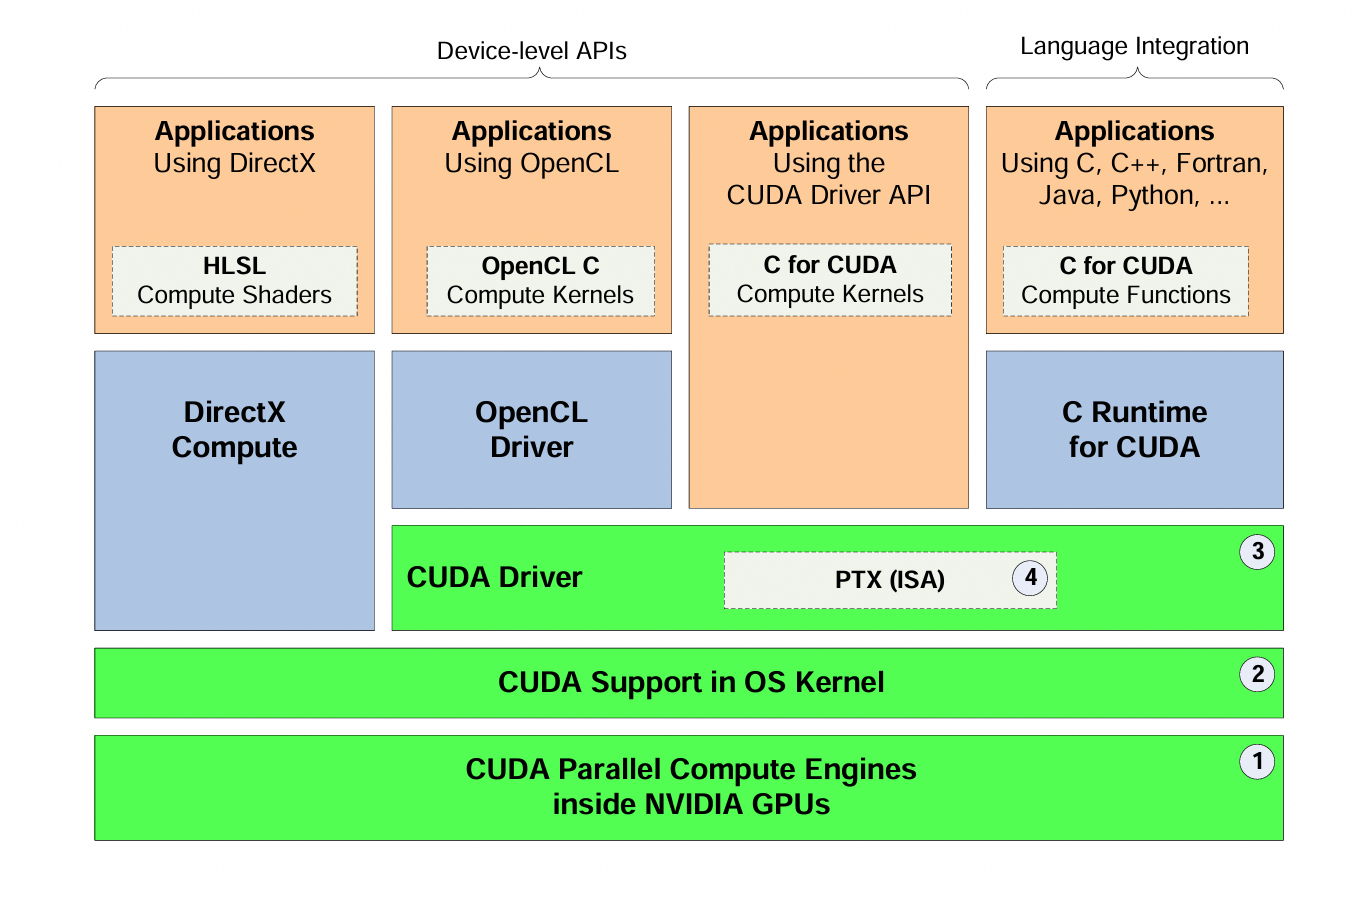
\includegraphics[width=0.85\textwidth]{images/figures/cuda-architecture.png}
    \caption{CUDA Architecture Overview}
    \label{fig: CUDA Architecture Overview}
\end{figure}

\subsubsection{Streaming Multiprocessors}
\label{subsubsec:sms}

The \acrfull{sm} is the fundamental autonomous execution unit of any NVIDIA
GPU. Each SM contains: CUDA cores (FP32/INT32 execution); Tensor Cores
(matrix multiply-accumulate, introduced in Volta 2017); warp schedulers
(typically 4 per SM); a large register file (32K–64K registers per SM
enabling zero-overhead context switching); configurable shared memory /
L1 cache (48–96 KB per SM); and special function units (SFUs) for
transcendental operations.

For reference, the NVIDIA A100 contains 108 SMs with 64 CUDA cores each
— totalling 6,912 cores — and can manage up to 2,048 threads per SM
simultaneously, grouped into 64 warps of 32 threads.

\subsubsection{SIMT Execution and Warp Model}
\label{subsubsec:simt}

CUDA implements the \acrfull{simt} model: groups of 32 consecutive threads
called \textit{warps} execute the same instruction in lock-step, each
operating on different data. Key properties of warp execution are:

\begin{itemize}
  \item All 32 threads in a warp execute the same instruction simultaneously.
  \item The warp scheduler switches between warps with zero overhead when
        one warp awaits memory — this is the primary latency-hiding mechanism.
  \item \textbf{Branch divergence}: when threads within a warp follow different
        execution paths, the warp serialises each path, potentially reducing
        throughput by up to 50\%.
  \item Each SM can manage 64 warps (2,048 threads) but dispatches typically
        4 warps per cycle through its warp schedulers.
\end{itemize}

% ── 2.1.2 ────────────────────────────────────────────────────
\subsection{CUDA Execution Model}
\label{subsec:cuda-execution}

\subsubsection{Thread Hierarchy}

CUDA organises threads into a two-level hierarchy. \textbf{Thread blocks}
are groups of threads that share data through shared memory and can
synchronise via barriers (\texttt{\_\_syncthreads()}). Block sizes are
multiples of 32 for warp alignment — typically 128, 256, or 512. A
\textbf{grid} is the collection of all thread blocks executing a kernel.
Each thread computes its unique global identifier as:
\begin{equation}
  i = \texttt{blockIdx.x} \times \texttt{blockDim.x} + \texttt{threadIdx.x}
  \label{eq:thread-id}
\end{equation}

\begin{figure}[H]
    \centering
    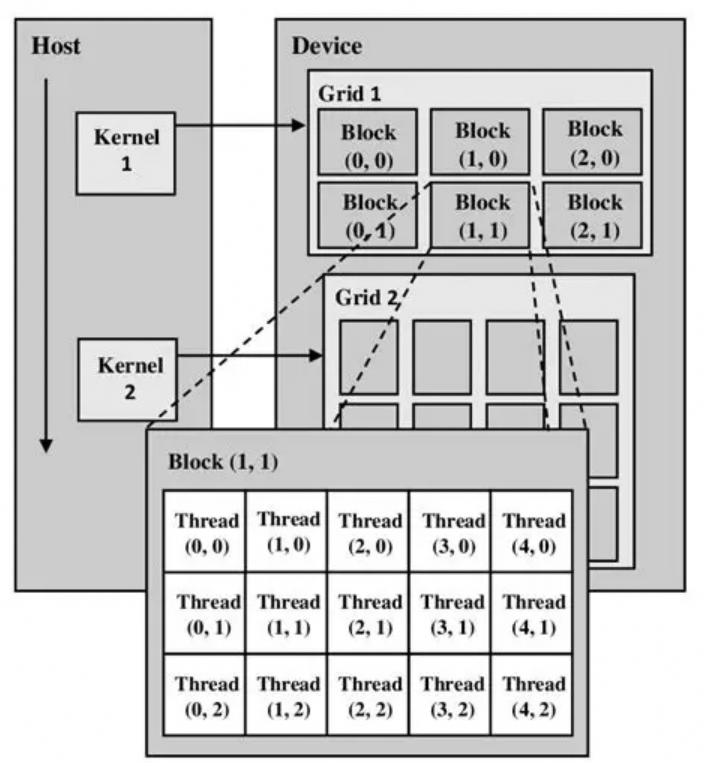
\includegraphics[width=0.85\textwidth]{images/figures/kernel-execution.png}
    \caption{Kernel Execution Flow}
    \label{fig:cuda-kernel-flow}
\end{figure}


% ── 2.1.3 ────────────────────────────────────────────────────
\subsection{CUDA Memory Hierarchy}
\label{subsec:cuda-memory}

CUDA exposes a multi-level memory hierarchy whose performance implications
are central to kernel optimisation. \tabref{cuda-memory} summarises the
key characteristics of each level.

\begin{table}[htbp]
  \centering
  \caption{CUDA memory hierarchy: latency, bandwidth, and scope}
  \label{tab:cuda-memory}
  \begin{tabularx}{\textwidth}{llllX}
    \toprule
    \tableheader{Memory Type & Scope & Capacity & Latency & Bandwidth} \\
    \midrule
    Registers      & Per-thread & $\sim$255 regs & $\sim$1 cycle  & $\sim$8 TB/s \\
    \rowcolor{TableRowOdd}
    Shared Memory  & Per-block  & 48–96 KB/SM  & 20–30 cycles & $>$1 TB/s \\
    L1 Cache       & Per-SM     & 16–48 KB/SM  & 20–30 cycles & $\sim$1 TB/s \\
    \rowcolor{TableRowOdd}
    L2 Cache       & Per-GPU    & 4–6 MB       & Tens of cycles & Moderate \\
    Global Memory  & Per-GPU    & 8–80 GB      & 400–800 cycles & 200–3,350 GB/s \\
    \rowcolor{TableRowOdd}
    Constant Mem.  & Per-GPU    & 64 KB        & $\sim$1 cycle (cached) & $\sim$800 GB/s \\
    \bottomrule
  \end{tabularx}
\end{table}

Three optimisation principles govern GPU memory performance. First,
\textbf{memory coalescing}: consecutive threads should access consecutive
addresses so the hardware merges accesses into fewer transactions —
strided access patterns can reduce effective throughput by 10–50$\times$.
Second, \textbf{shared memory tiling}: caching frequently reused data in
shared memory (20–30 cycle latency) avoids repeated 400–800 cycle global
memory round-trips, which is critical for tiled matrix multiplication and
convolution. Third, \textbf{register pressure}: excessive register usage
reduces occupancy (active warps per SM), limiting the scheduler's ability
to hide global memory latency — maintaining above 50\% occupancy is
typically the target.

% ── 2.1.4 ────────────────────────────────────────────────────
\subsection{CUDA Ecosystem and Software Stack}
\label{subsec:cuda-ecosystem}

CUDA's dominance in AI infrastructure is as much a software phenomenon as
a hardware one. The CUDA Toolkit provides a complete development
environment: the \texttt{nvcc} compiler, profiling tools (Nsight Systems,
Nsight Compute), and a suite of hand-tuned libraries summarised in
\tabref{cuda-libs}.

\begin{figure}[H]
    \centering
    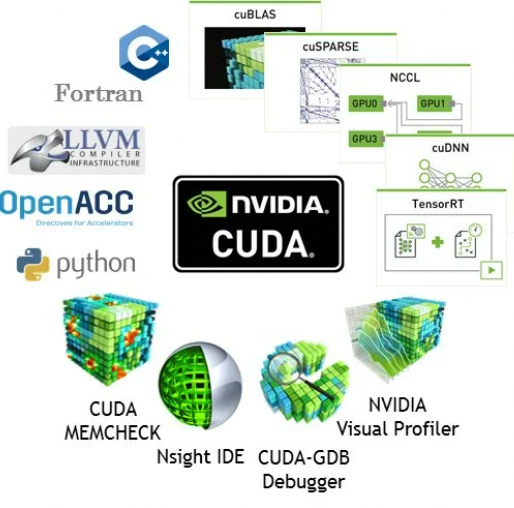
\includegraphics[width=0.85\textwidth]{images/figures/cuda-ecosystem.png}
    \caption{CUDA Ecosystem Overview}
    \label{fig:cuda-ecosystem}
\end{figure}

\begin{table}[htbp]
  \centering
  \caption{Core CUDA libraries and their relevance to AI workloads}
  \label{tab:cuda-libs}
  \begin{tabularx}{\textwidth}{llX}
    \toprule
    \tableheader{Library & Function & AI Relevance} \\
    \midrule
    cuDNN    & Deep neural network primitives & Conv, pooling, normalisation, RNN; 5–10$\times$ speedup \\
    \rowcolor{TableRowOdd}
    cuBLAS   & Basic linear algebra           & Matrix multiplication for all linear layers \\
    NCCL     & Collective communications       & Multi-GPU gradient synchronisation \\
    \rowcolor{TableRowOdd}
    TensorRT & Inference optimisation          & Layer fusion, quantisation; 3–5$\times$ faster inference \\
    CUTLASS  & Templated GEMM kernels          & Custom matrix operations for novel architectures \\
    \bottomrule
  \end{tabularx}
\end{table}

PyTorch and TensorFlow achieve GPU acceleration by dispatching operations to
these libraries rather than implementing custom kernels. Over 95\% of papers
at top AI venues (NeurIPS, ICML, ICLR) use NVIDIA GPUs, creating
reproducibility norms that reinforce adoption and make CUDA the path of
least resistance for AI researchers and engineers.

This dominance, however, creates structural risks: CUDA is NVIDIA-exclusive;
migration to ROCm, oneAPI, or CANN requires substantial re-engineering;
and library optimisations are often CUDA-first — sometimes CUDA-only. These
factors create the vendor lock-in dynamic that motivates the exploration of
alternative ecosystems examined in subsequent chapters.
